%%%%%%%%%%%%%%%%%%%%%%%%%%%%%%%%%%%%%%%%%%%%%%%%%%%%%%%%%%%%%%%%%%%%%%%%%%%%%%%%
% Thesis / Project Report
% LaTeX Template
% Version 2.0 (08/04/16)
%
% Author:
% Siddhant Shrivastava
% https://github.com/sidcode/bits-pilani-thesis-template-latex
%
% This template is heavily based on the work of Darshit Shah, Steven Gunn and Sunil Patel
% Darshit Shah
% https://github.com/darnir/BPHC-LaTeX-Report-Class
% Steven Gunn
% http://users.ecs.soton.ac.uk/srg/softwaretools/document/templates/
% and
% Sunil Patel
% http://www.sunilpatel.co.uk/thesis-template/
%
% License:
% CC BY-NC-SA 4.0 (http://creativecommons.org/licenses/by-nc-sa/4.0/)
%
% Note:
% Make sure to edit document variables in the Thesis.cls file
%
%%%%%%%%%%%%%%%%%%%%%%%%%%%%%%%%%%%%%%%%%%%%%%%%%%%%%%%%%%%%%%%%%%%%%%%%%%%%%%%%

%-------------------------------------------------------------------------------
%	PACKAGES AND OTHER DOCUMENT CONFIGURATIONS
%-------------------------------------------------------------------------------

\documentclass[12pt, a4paper, oneside]{Thesis} % Paper size, default font size
                                               % and one-sided paper

\graphicspath{{Pictures/}} % Specifies the directory where pictures are stored

%\usepackage[backend=bibtex]{biblatex}
%\bibliography{Bibliography.bib}


\usepackage{bm}
\usepackage{amsmath}
\usepackage{float}
\usepackage{tikz,pgfplots}
	\usetikzlibrary{datavisualization}
	\usetikzlibrary{datavisualization.formats.functions}
\usepackage{color}
	\definecolor{dkgreen}{rgb}{0,0.6,0}
	\definecolor{gray}{rgb}{0.5,0.5,0.5}
	\definecolor{mauve}{rgb}{0.58,0,0.82}
\usepackage{listings}
	\lstset{frame=tb,
	  language=Python,
	  aboveskip=3mm,
	  belowskip=3mm,
	  showstringspaces=false,
	  columns=flexible,
	  basicstyle={\small\ttfamily},
	  numbers=none,
	  numberstyle=\tiny\color{gray},
	  keywordstyle=\color{blue},
	  commentstyle=\color{dkgreen},
	  stringstyle=\color{mauve},
	  breaklines=true,
	  breakatwhitespace=true,
	  tabsize=3
	}
\title{\ttitle} % Defines the thesis title - don't touch this

\begin{document}

\frontmatter % Use roman numbering style (i, ii...) for the pre-content pages

\setstretch{1.1} % Line spacing of 1.1

% Define page headers using FancyHdr package and set up for one-sided printing
\fancyhead{} % Clears all page headers and footers
\rhead{\thepage} % Sets the right side header to show the page number
\lhead{} % Clears the left side page header

\pagestyle{fancy} % Finally, use the "fancy" page style to implement the
                  %FancyHdr headers

% Input all the variables used in the document. Please fill out the
% variables.tex file with all your details.
%-------------------------------------------------------------------------------
%	DOCUMENT VARIABLES
%
%	Fill in the lines below to set the various variables for the document
%-------------------------------------------------------------------------------

%-------------------------------------------------------------------------------
% Your thesis title - this is used in the title and abstract
% Command: \ttitle
\thesistitle{Augmented Reality using Deep Learning for Scene Understanding}
%-------------------------------------------------------------------------------
% The document type: Thesis / report, etc.
% Command: \doctype
\documenttype{Project Report}
%-------------------------------------------------------------------------------
% Your supervisor's name - this is used in the title page
% Command: \supname
\supervisor{Prof. Tathagata \textsc{Ray}}
%-------------------------------------------------------------------------------
% The supervisor's position - Used on Certificate
% Command: \suppos
\supervisorposition{Associate Professor}
%-------------------------------------------------------------------------------
% Supervisor's institute
% Command: \supinst
 \supervisorinstitute{BITS Pilani, Hyderabad Campus}
%-------------------------------------------------------------------------------
% Your Co-Supervisor's name
% Command: \cosupname
% \cosupervisor{Dr. N L \textsc{Bhanumurthy}}
%-------------------------------------------------------------------------------
% Co-Supervisor's Position - Used on Certificate
% Command: \cosuppos
% \cosupervisorposition{Asst. Professor}
%-------------------------------------------------------------------------------
% Co-Supervisor's Institute
% Command: \cosupinst
%\cosupervisorinstitute{BITS Pilani, Hyderabad Campus}
%-------------------------------------------------------------------------------
% Your Examiner's name. Not currently used anywhere.
% Command: \examname
\examiner{}
%-------------------------------------------------------------------------------
% Name of your degree
% Command: \degreename
\degree{Bachelor of Engineering (Hons.)}
%-------------------------------------------------------------------------------
% The BITS Course Code for which this report is written
% COmmand: \ccode
\coursecode{BITS F376}
%-------------------------------------------------------------------------------
% The name of the Course
% Command: \cname
\coursename{Design Oriented Project}
%-------------------------------------------------------------------------------
% Your name. Extend manually in case of multiple authors
% Command: \authornames
\authors{Adityakrishna \textsc{Chivukula}}
%-------------------------------------------------------------------------------
% Your ID Number - used on the Title page and abstract
% Command: \idnum
\IDNumber{2013A7TS387H}
%-------------------------------------------------------------------------------
% Your address
% Command: \addressnames
\addresses{}
%-------------------------------------------------------------------------------
% Your subject area
% Command: \subjectname
\subject{}
%-------------------------------------------------------------------------------
% Keywords for this report.
% Command: \keywordnames
\keywords{}
%-------------------------------------------------------------------------------
% University details
% Command: \univname
\university{\texorpdfstring{\href{http://www.bits-pilani.ac.in/} % URL
                {Birla Institute of Technology and Science Pilani}} % University name
                {Birla Institute of Technology and Science Pilani}}
%-------------------------------------------------------------------------------
% University details, in Capitals
% Command: \UNIVNAME
\UNIVERSITY{\texorpdfstring{\href{http://www.bits-pilani.ac.in/} % URL
                {BIRLA INSTITUTE OF TECHNOLOGY AND SCIENCE PILANI}} % name in capitals
                {BIRLA INSTITUTE OF TECHNOLOGY AND SCIENCE PILANI}}

%-------------------------------------------------------------------------------
% Campus Name
% Command: \campusname
\campus{Hyderabad Campus}

%-------------------------------------------------------------------------------
% Campus Name, in capitals
% Command: \CAMPUSNAME
\CAMPUS{HYDERABAD CAMPUS}


%-------------------------------------------------------------------------------
% Department Details
% Command: \deptname
\department{\texorpdfstring{\href{http://www.bits-pilani.ac.in/pilani/computerscience/ComputerScience} % Your department's URL
                {Computer Science \& Information Systems}} % Your department's name
                {Computer Science}}
%-------------------------------------------------------------------------------
% Department details, in Capitals
% Command: \DEPTNAME
\DEPARTMENT{\texorpdfstring{\href{http://www.bits-pilani.ac.in/pilani/computerscience/ComputerScience} % Your department's URL
                {COMPUTER SCIENCE \& INFORMATION SYSTEMS}} % Your department's name in capitals
                {COMPUTER SCIENCE \& INFORMATION SYSTEMS}}
%-------------------------------------------------------------------------------
% Research Group Details
% Command: \groupname
\group{\texorpdfstring{\href{Research Group Web Site URL Here (include http://)}
                {Research Group Name}} % Your research group's name
                {Research Group Name}}
%-------------------------------------------------------------------------------
% Research Group Details, in Capitals
% Command: \GROUPNAME
\GROUP{\texorpdfstring{\href{Research Group Web Site URL Here (include http://)}
                {RESEARCH GROUP NAME (IN BLOCK CAPITALS)}}
                {RESEARCH GROUP NAME (IN BLOCK CAPITALS)}}
%-------------------------------------------------------------------------------
% Faculty details
% Command: \facname
\faculty{\texorpdfstring{\href{Faculty Web Site URL Here (include http://)}
                {Faculty Name}}
                {Faculty Name}}
%-------------------------------------------------------------------------------
% Faculty details, in Capitals
% Command: \FACNAME
\FACULTY{\texorpdfstring{\href{Faculty Web Site URL Here (include http://)}
                {FACULTY NAME (IN BLOCK CAPITALS)}}
                {FACULTY NAME (IN BLOCK CAPITALS)}}
%-------------------------------------------------------------------------------


%-------------------------------------------------------------------------------
%   NON-CONTENT PAGES
%-------------------------------------------------------------------------------
\maketitle
\Declaration
\Certificate
% \Quotation{Insert Random Quote here. Publish like a boss.}{Your Name}

\begin{abstract}
Neural Networks have surpassed human-level accuracy in several classification and recognition tasks over the past few years. This unprecedented performance is attributed to improvement in algorithms, access to larger datasets, higher computational power and better theoretical understanding of high dimension statistics. The latest wave of performance increase of Neural Networks has been branded deep learning on account of the depth of the novel networks that learn the data representations. Through the course of this report, I intend to analyse the factors stated above and how they individually contributed to the development of the field into the forerunner for achieving Artificial General Intelligence.
\end{abstract}

\begin{acknowledgements}
I would like to thank \supname{} and the Department of Computer Science for the opportunity and resources to pursue this project.
\end{acknowledgements}

%-------------------------------------------------------------------------------
%	LIST OF CONTENTS/FIGURES/TABLES PAGES
%-------------------------------------------------------------------------------

% The page style headers have been "empty" all this time, now use the "fancy"
% headers as defined before to bring them back
\pagestyle{fancy}

\lhead{\emph{Contents}} % Set the left side page header to "Contents"
\tableofcontents % Write out the Table of Contents

% Set the left side page header to "List of Figures"
% \lhead{\emph{List of Figures}}
% \listoffigures % Write out the List of Figures

 % Set the left side page header to "List of Tables"
% \lhead{\emph{List of Tables}}
% \listoftables % Write out the List of Tables

%-------------------------------------------------------------------------------
%	ABBREVIATIONS
%-------------------------------------------------------------------------------

%\clearpage % Start a new page

 % Set the line spacing to 1.5, this makes the following tables easier to read
%\setstretch{1.5}

%\lhead{\emph{Abbreviations}} % Set the left side page header to "Abbreviations"
%\listofsymbols{ll} % Include a list of Abbreviations (a table of two columns)
%{
%$\hat{\bm{y}}$ & Labeled class/output for training example \\
%\textbf{Acronym} & \textbf{W}hat (it) \textbf{S}tands \textbf{F}or \\
%}

%-------------------------------------------------------------------------------
%	PHYSICAL CONSTANTS/OTHER DEFINITIONS
%-------------------------------------------------------------------------------

%\clearpage % Start a new page

% Set the left side page header to "Physical Constants"
%% \lhead{\emph{Physical Constants}}

 % Include a list of Physical Constants (a four column table)
%% \listofconstants{lrcl}
%%{
%%Speed of Light & $c$ & $=$ & $2.997\ 924\ 58\times10^{8}\ \mbox{ms}^{-\mbox{s}}$ (exact)\\
%% Constant Name & Symbol & = & Constant Value (with units) \\
%%}

%-------------------------------------------------------------------------------
%	SYMBOLS
%-------------------------------------------------------------------------------

%\clearpage % Start a new page

%\lhead{\emph{Glossary}} % Set the left side page header to "Symbols"

%\listofnomenclature % List the nomenclature. (We use the glossaries package)

%-------------------------------------------------------------------------------
%	DEDICATION
%-------------------------------------------------------------------------------

\setstretch{1.1} % Return the line spacing back to 1.3

%%\pagestyle{empty} % Page style needs to be empty for this page

% Dedication text
%%\Dedicatory{Dedicate this to someone, anyone.}

%%\addtocontents{toc}{\vspace{2em}} % Add a gap in the Contents, for aesthetics


%-------------------------------------------------------------------------------
%	THESIS CONTENT - CHAPTERS
%-------------------------------------------------------------------------------

\mainmatter % Begin numeric (1,2,3...) page numbering

\pagestyle{fancy} % Return the page headers back to the "fancy" style

% Include the chapters of the thesis as separate files from the Chapters folder
% Uncomment the lines as you write the chapters

% Chapter 1

\chapter{Introduction} % Main chapter title

\label{intro} % For referencing the chapter elsewhere, use \ref{Chapter1} 

\lhead{Chapter 1. \emph{Introduction}} % This is for the header on each page - perhaps a shortened title

%----------------------------------------------------------------------------------------

Deep learning provides a very powerful framework to perform supervised learning. Adding more layers and more units within a layer, a deep network can represent functions of great complexity. It is proven that Neural Networks are Universal function approximators. Therefore with networks of sufficient size and with data and computational power to match, tasks that consist of mapping an input vector to an output vector, and that are easy for a person to do rapidly, can be accomplished via deep learning, given labeled training examples.

\section*{History}
Neural Networks, as the name suggest was inspired by modeling of the brain functions. The earliest ancestor of these networks was the \textit{multi-layer perceptron}. It represented a linear classifier that had individual perceptrons firing to indicate location of the test point on the higher-dimension space decision boundary.

%\section*{Recent Developments}



% Chapter 2

\chapter{Requisite Mathematics} % Main chapter title
\label{ch:math} % For referencing the chapter elsewhere, use \ref{Chapter1} 

\lhead{Chapter 2. \emph{Requisite Mathematics}} % This is for the header on each page - perhaps a shortened title

%----------------------------------------------------------------------------------------

This chapter presents some of the basic math involved in constructing and training Deep Learning models. The concepts presented in this chapter assume few results from Linear Algebra and Probability Theory.  Further, we will consider the numerical computation issues that come into play while implementing the theory in practice. an attempt to develop some intuition about the high-dimensional statistics involved in the trained models is presented in the last section.

\section{Backpropogation and Automatic Differentiation}
\label{sec:bpad}
The invention of the backpropagation algorithm was the turning point in the history of Neural Networks. It allowed efficient computation of the gradients of the cost function with respect to all the parameters in the model. For any \textit{unrolled} set of parameters. We need to calculate the partial derivatives of the cost $J$ with respect to each $\theta _{i} \in \bm{\theta}$. The function J is given by,
\begin{equation}
J(\bm{x},\bm{\hat{y}};\bm{\theta}) = L(f(\bm{x};\bm{\theta}), \bm{\hat{y}})
\end{equation}
Therefore, the gradients we need to determine are:
\begin{equation}
\nabla _{\bm{\theta }} J \frac{\partial J }{\partial \bm{ \theta }}
\end{equation}

The choice of the loss function $L$ is elaborated in the next section.

Automatic Differentiation can be viewed as the generalised version of backpropagation. The fundamental concept is the application of chain rule at the operator level, for the evaluation of the gradient. We setup a computational graph as a composition of primitive operations. Every node takes multiple variables as arguments and has outputs. The chain rule states that the gradient with resepct to the output can be split in terms of the input.

Ex.
\begin{align*}
L &= x + y			&		L &= x * y \\
\frac{\partial L}{\partial x} &= 1 & \frac{\partial L}{\partial x} &= y\\
\frac{\partial L}{\partial y} &= 1 & \frac{\partial L}{\partial y} &= x
\end{align*}

\section{Loss Functions}

Loss functions determine the error that backpropagates through the network. It quantifies the error produced by the network on a training sample with reagrd to the labeled target value.

\subsection*{Euclidean Distance / Mean-Squared Error (MSE)}
The plain vanilla Euclidean distance of the $L^2$ norm can be used to measure the error between output vectors. Use of this function is not practical in large networks as the gradient explodes due the quadratic nature of the curve.
\begin{equation}
J(\hat{\bm{y}},f(\bm{x};\bm{\theta})) = ||\hat{\bm{y}} - f(\bm{x};\bm{\theta})||^{2}
\end{equation}
where $f(\bm{x};\bm{\theta})$ is the output from the model and $\bm{y}$ is the labeled target for the training example.





\subsection*{Cross-Entropy Loss}
When we have two separate probability distributions $P(\bm{x})$, $Q(\bm{x})$ defined over the same random variable $\bm{x}$, we can define the \textit{divergence} of the pair of distributions. It is a measure of how dissimilar the two probability distributions are. Information theory provides a useful method of measuring this divergence called \textit{Kullback-Leibler (KL) divergence}:
\begin{equation}
\label{eq:celoss}
D_{KL}(P \parallel Q) = E_{x \sim P}\left[log \frac{P(\bm{x})}{Q(\bm{x})}\right]
\end{equation}
Some immediate properties that become evident from this equation are that the value of $D_{KL}(P\parallel Q) = 0$ only if $P(\bm{x})$ and $Q(\bm{x})$ are the same probability distribution. Further, the divergence measured is always non-negative and can be interpreted as a type of distance metric, much like Euclidean distance. Notice however that $D_{KL}(P \parallel Q) \neq D_{KL}(Q \parallel P)$. Therefore KL divergence is not a symmetric operation. This brings us to our definition of \textit{cross-entropy loss},
\begin{equation}
H(P,Q) = H(P) + D_{KL}(P \parallel Q)
\end{equation}
From Eq.\ref{eq:celoss}, it can be seen that this is equivalent to,
\begin{equation}
H(P,Q) = -E_{x \sim P}\left[ \log Q(\bm{x})\right]
\end{equation}
Therefore, minimizing the cross-entropy loss is w.r.t. $Q$ is equivalent to minimizing the KL divergence. This makes sense intuitively since we want the distribution of the laebelled target value $\hat{\bm{y}}$ to match the output of the model $f( \bm{x} ; \bm{ \theta } )$ Also, the output allows for a probabilistic interpretation of the output vector.
\section{Activation Functions}
Activation Functions are in a sense the essence of the functionality of Neural Networks, they introduce the non-linearities that allow the network to learn the complex decision boundaries in high dimension space (discussed in sec.\ref{sec:highds}) Our choice of activation ffunction is guided by the following considerations:
\begin{itemize} \itemsep -3pt
\item Saturation of function for high input value i.e. vanishing gradient.
\item Centering of values around zero for even distribution of activations.
\end{itemize}
We evaluate the following functions based on these two considerations along with explanations for the requirements.

\subsection*{Sigmoid}
 The sigmoid function $\sigma(\bm{x})$ is defined as $\sigma(\bm{x}) = 1/1+e^{-\bm{x}}$. This activation was traditionally the de facto non-linearity added to hidden layers as it resembled the firing of a biological neuron i.e. \textit{zero} being inactive and \textit{one} being active/firing. THe sigmoid function had worked relatively well for training neural networks for a long time, but posed an important issue for the larger models. several coumpounded activations over multiple layers led to the \textit{saturation} of the neuron. This means that the value of the function at $\mod 3 $ is at $0.95$. As you can notice, the gradient of the graph also tends to zero beyond these points. We require the gradient to be non-zero for all segments of the firing of the neuron, as the error information back propagates through all layers via the activation value as explained in sec.\ref{sec:bpad}. \\

\begin{figure}[H]
	\centering
	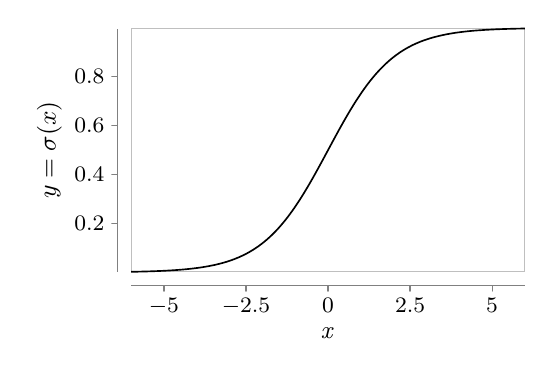
\begin{tikzpicture}

	\datavisualization [scientific axes=clean,
                    visualize as smooth line,
                    y axis={label={$y= \sigma (x)$}},
                    x axis={label} ]

	data [format=function] {
      var x : interval [-6:6] samples 100;
      func y = 1 / (1 + exp( -1 * \value x ));
      };
	\end{tikzpicture}
\caption{Sigmoid activation function}
\label{fig:sigm}
\end{figure}

The sigmoid function was popular due to the convenience of representing its gradient in terms of itself, i.e.
\begin{align*}
\sigma(x) &= \frac{1}{1 + e^{-x}}\\
\frac{\partial \sigma }{\partial x} &= \frac{e^{-x}}{1+e^{-x}} = (\sigma (x)\left(1-\sigma (x)\right)\\
\end{align*}

\subsection*{Hyperbolic Tangent}

\begin{figure}[H]
	\centering
	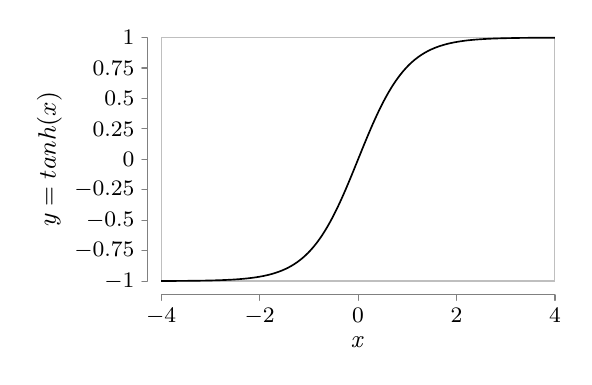
\begin{tikzpicture}
	\datavisualization [scientific axes=clean,
                    visualize as smooth line,
                    y axis={label={$y=tanh(x)$}},
                    x axis={label} ]

	data [format=function] {
      var x : interval [-4:4] samples 100;
      func y = (1 - exp( -2 * \value x))/(1 + exp( -2 * \value x));
      };
	\end{tikzpicture}
\caption{Hyperbolic tangent activation fnction}
\label{fig:tanh}
\end{figure}
\begin{align*}
tanh(x) &= \frac{1 - e^{-2x}}{1 + e^{-2x}}\\
\frac{\partial tanh(x) }{\partial x} &= 1 - tanh(x)^2
\end{align*}
\begin{figure}[H]
	\centering
	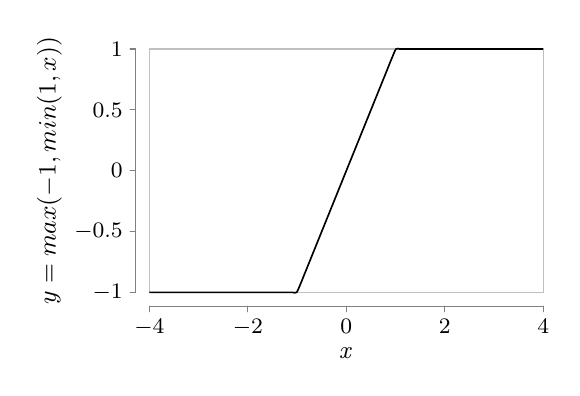
\begin{tikzpicture}
	\datavisualization [scientific axes=clean,
                    visualize as smooth line,
                    y axis={label={$y=max( -1, min( 1, x))$}},
                    x axis={label} ]

	data [format=function] {
      var x : interval [-4:4] samples 100;
      func y = max( -1, min( 1, \value x));
      };
	\end{tikzpicture}
\caption{Hard Hyperbolic tangent activation fnction}
\label{fig:tanh}
\end{figure}

\subsection*{Rectified Lineinar Unit (ReLU)}

\begin{figure}[H]
	\centering
	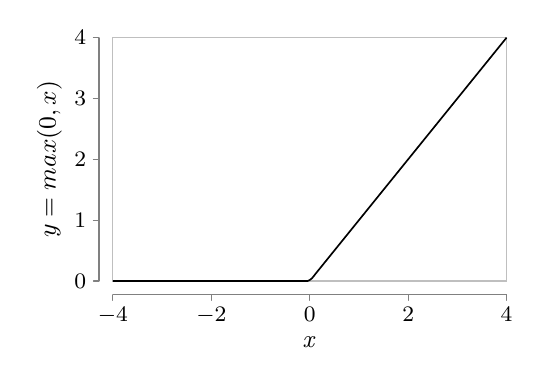
\begin{tikzpicture}
	\datavisualization [scientific axes=clean,
                    visualize as smooth line,
                    y axis={label={$y=max(0,x)$}},
                    x axis={label} ]

	data [format=function] {
      var x : interval [-4:4] samples 100;
      func y = max( 0, \value x);
      };
	\end{tikzpicture}
\caption{ReLU activation function}
\label{fig:relu}
\end{figure}

\begin{align*}
 o(x) &= max(0,x)\\
\frac{\partial o(x) }{\partial x} &= 1, x > 0 & 0, x \le 0
\end{align*}

\begin{figure}[H]
	\centering
	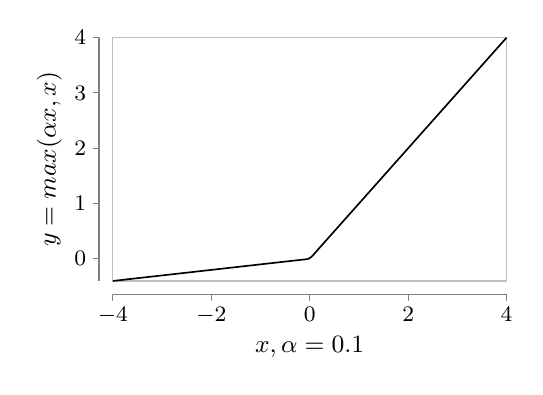
\begin{tikzpicture}
	\datavisualization [scientific axes=clean,
                    visualize as smooth line,
                    y axis={label={$y=max(\alpha x,x)$}},
                    x axis={label={$x, \alpha = 0.1$}} ]

	data [format=function] {
      var x : interval [-4:4] samples 100;
      func y = max( 0.1 * \value x, \value x);
      };
	\end{tikzpicture}
\caption{Leaky ReLU activation function}
\label{fig:lrelu}
\end{figure}



\subsection*{Softplus}

\begin{figure}[H]
	\centering
	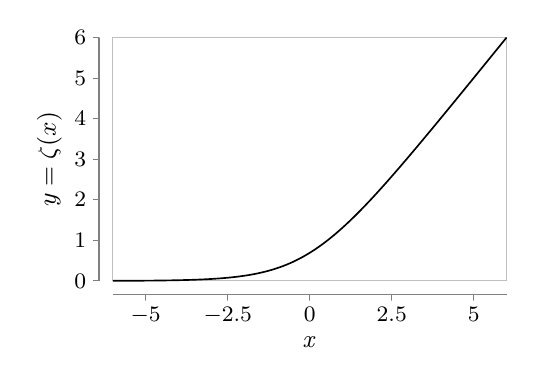
\begin{tikzpicture}

	\datavisualization [scientific axes=clean,
                    visualize as smooth line,
                    y axis={label={$y= \zeta (x)$}},
                    x axis={label} ]

	data [format=function] {
      var x : interval [-6:6] samples 100;
      func y = ln(1 + exp( \value x ));
      };
	\end{tikzpicture}
\caption{softplus activation function}
\label{fig:sigm}
\end{figure}

\section{Optimisation}

\begin{figure}[H]
	\centering
	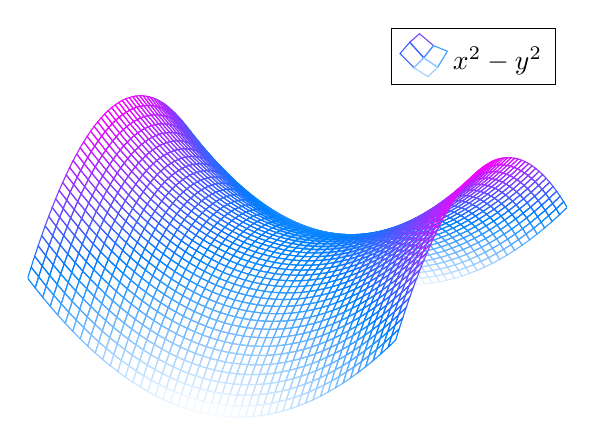
\begin{tikzpicture}
	\begin{axis}[
	    hide axis,
	    colormap/cool,
	]
	\addplot3[
	    mesh,
	    samples=50,
	    domain=-8:8,
	]
	{(x^2-y^2)};
	\addlegendentry{$x^2 - y^2$}
	\end{axis}
	\end{tikzpicture}
\caption{Saddle Point}
\label{fig:sadp}
\end{figure}

\begin{figure}[H]
	\centering
	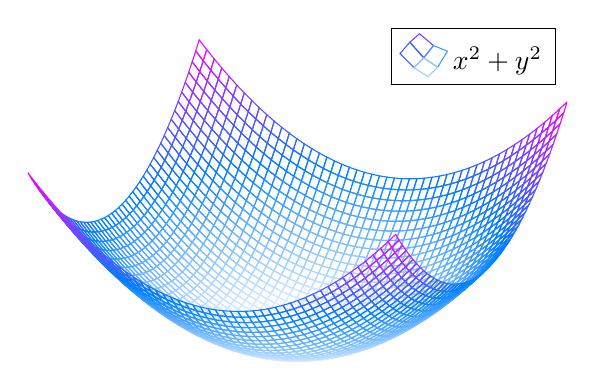
\begin{tikzpicture}
	\begin{axis}[
	    hide axis,
	    colormap/cool,
	]
	\addplot3[
	    mesh,
	    samples=50,
	    domain=-8:8,
	]
	{(x^2+y^2)};
	\addlegendentry{$x^2 + y^2$}
	\end{axis}
	\end{tikzpicture}
\caption{Minima}
\label{fig:minp}
\end{figure}

\subsection*{Stochastic Gradient Descent and its variants}
Stochastic Gradient Descent is the de facto method for training any Neural Network. The basic equation for the parameter updates using SGD is give by,
\begin{equation}
\theta_ i := \theta_i - \alpha \frac{\partial J}{\partial \theta_i}
\end{equation}
\subsection*{Comparison}

\begin{figure}[H]
	\centering
	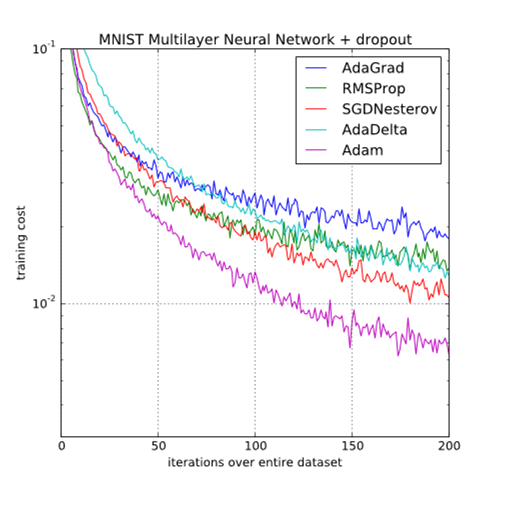
\includegraphics[scale=0.4]{Pictures/convergrate.png}
	\rule{35em}{0.5pt}
	\caption[gd]{Convergence rates of various Gradient Descent algorithms.}
	\label{fig:converg}
\end{figure}





% Chapter 1

\chapter{Neural Networks Architectures} % Main chapter title

\label{nnarch} % For referencing the chapter elsewhere, use \ref{Chapter3} 

\lhead{Chapter 3. \emph{Neural Networks Architectures}} % This is for the header on each page - perhaps a shortened title

%----------------------------------------------------------------------------------------
This chapter will explore the ways to construct a Neural Network. We will develop some basic elements (i.e. Neurons and Layers) that can combined in several ways, much like a child's toy building bricks to design large netowkrs capable of representing complex functions. We will also present the various ways of interpreting the working of a such networks and seek to apply these empirically developed intuitive rules to provide general guidelines while using the networks in practice.\\

An important result of the late 20th century was the proof by Hornik et al., that a feedforward network with a linear output layer containing at least one hidden layer, and any activation function, which non-linearly constrains the output of each neuron to lie in a finite range (such as
the logistic sigmoid activation function), can approximate any Borel measurable
function. The Borel measurable function, for purposes of the discussion loosely qualifies as a continuous and differentiable function. The paper further shows that there exists a network that can approximate the function mapping from one finite-dimension space to another, to any level desired level of accuracy (based on the number of hidden units). However, it does not tell us how. Empirically, it can be shown that certain functions require exponential number of hidden units (w.r.t to number traning examples) to learn the functino approximation. It sufficies to say that the feedforward network aims to learn $\bm{y}=\bm{f^{*}}(\bm{x})$ that best approximates the function $\bm{f}$. Moreover, the proof doesn't provide any information on the trainability of such networks. Which is a crucial factor in designing large scale deployable models.

\section{Feedforward Neural Networks}

Feedforward Networks are the basis of all current deep learning techniques. The goal of such a network is to approximate a classifier, $\bm{y}=\bm{f}^{*}(\bm{x})$.These networks are essentially Directed Acyclic Graphs and are called \textit{feedforward} as the computations behave as a flow of data through a composition of sub-functions to compute the classifier function that the network learns. The remainder of the section aims to analyse and understand the behaviour of the composition and flow of data through the model.\\


\section{Convolutional Neural Networks (CNNs)}

CNNs are a unique architecture of networks that are used to process mainly images in computer vision tasks. It also used on other interesting types of data such as, time series data and sequential data. The main property of these networks is the ability to create \textit{feature maps} that a re a consequence of the convolution operation. Broadly, any network that uses a convolution operation in placae of the standard matrix multiply in fully connected layers may be termed as a CNN.

\subsection*{Convolution Operation}
The convolution operation is defined as the following,
\begin{equation}
s(t) = \int x(a)w(t-a)da
\end{equation}
\begin{equation}
s(t) = (x*w)(t)
\end{equation}
$w$ is a weighting function that is interpreted as the weight assigned to the history of the function $p$. $w$ is constrained to be a valid probability distribution and also must be 0 for negative values od $a$. 
The discrete version of this operation is given by,
\begin{equation}
s(t) = (x*w)(t) = \sum_{a=-\infty}^{\infty}x(a)w(t-a)
\end{equation}
In the context computer vision, the equation takes a slightly different form to account for images being 2D grids of pixel values.
\begin{equation}
\label{eq:conv}
S(i,j) = (I*K)(i,j) = \sum_m \sum_n I(m,n)K(i-m,j-n)
\end{equation}
Convolution operation is defined to be commutative, therefore Eq.\ref{eq:conv} is the same as,
\begin{equation}
S(i,j) = (K*I)(i,j) = \sum_m \sum_n I(i-m, j-n)K(m,n)
\end{equation}
From this equation, we call the function K to be a \textit{filter}, and the output $\bm(S)$ convolved over the entire input $(i,j)$ and extracted feature map. The strategy of applying filters over each subsequent layer to produce multiple feature maps allow representing the image data in a new \textit{topologically equivalent} representation space over which a classifier, such as a full-connected neural network layer or a SVM can be learnt. These learnt classifiers can be shaped to necessary dimension to conform with the available labeled target values $\bm{\hat{y}}$ to calculate the loss corresponding to each training example. The loss can now be backpropagated through the network to learn the network parameters that accurately classify the train data available.

\begin{figure}[H]
		\centering
		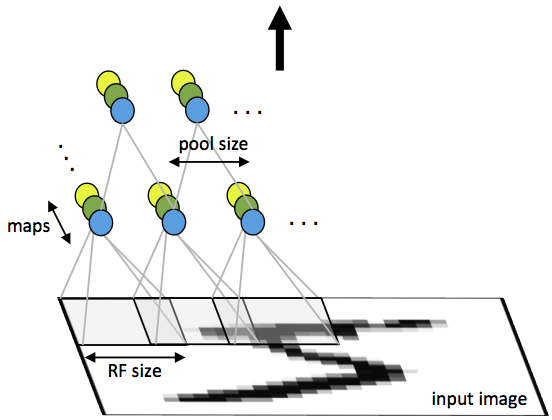
\includegraphics[scale=0.4]{Pictures/cnn.png}
		\rule{35em}{0.5pt}
		\caption[Convolutional Neural Network]{Convolutional Neural Network.}
		\label{fig:rnn}
\end{figure}

Further subsections discuss the considerations that go into designing these convolutional networks structures as well as optimisation and trainability conditions.
\subsection*{Filters}
The area covered by a filter (measured in pixel units) is called the \textit{receptive field size}. THe input image can be viewed as a volume of image size times the individual RGB values. So for an image of width $w$ and height $h$. The input volume would be $w*h*d$, where $d=3$ corresponding to each channel RGB. After applying $n$ filters of size $k*k$ each, we generate a layer of feature values of size $(w-k+1)*(h-k+1)*n$. Some methods of \textit{data augmentation} include adding of padded zeroes around the image that allow the filter to be applied in a manner that produce the same width and height dimensions for the output as the given input. This is useful for segmentation tasks discussed in the later sections.

The variable in this method of application of convolutions has three main variables.
\begin{itemize} \itemsep -2pt
\item \textit{Number of layers:} We can apply several layers of convolutional to generate intermediate representations of greater complexity. However greater complexity does not translate to better quality.  We can notice from the structure of the convolutional layers that the output of filters closer to the image data have a small receptive field, as the depth of the network increase, the output of every neuron is a function of a much larger area of the input image.
\item \textit{Dimension of filters:} The value of $k$ can be changed to modify the receptive field of each filter applied on the output of previous layers. While intuitively it might seem like a better idea to increase the receptive field size. It is shown experimentally that a larger filter dimension inhibits performance of the network. The added incentive of using smaller filter dimensions is the computational consideration. Due to the ability to parallelize the networks (discussed in sec.\ref{sec:impl}), smaller filters require lesser computation.
\item \textit{Number of filters per layer:} Every new feature map volume has a depth corresponding to the number of filters in the previous convolutional layer. Each filter is expected to behave as a unique feature detector from the repesentation space of the previous layer. The number of filters in each layer is an approximation of the number of features we expect to see in that layer. The output of a particular filter neuron is considered active if that feature is detected in the sub-volume equal to the receptive field size of that filter. Large number of filters cause the intermediate representation volumes to become very large. A pooling operation reduces the dimensionality of these volumes. It is essential to use a pool operation regardless of the input volume size for reasons discussed in the next section.
\end{itemize}

\subsection*{Pool}

As discussed in the earlier section, Every layer of applying convolutional filters creates a new \textit{volume}. Over subsequent layers these volumes can tend to become very large and store redundant data representations. Both issues are tackled by occasionaly including a \textit{pool} layer in between concolutional layers. A pool operation is applied to specific non-overlapping sub-volumes to produce a single output. This reduces the dimensionality of the input volume to each layer. Pooling also helps to make the representation become relatively invariant to small translations of the input. Invariance to translation implies that spatial displacement of lower level features will not affect the feature map of higher levels. This is desirable if the task to be performed is dependant on the existance of features rather than the location of the said features.

Some of the pool operations that are used are, \textit{max-pool}, \textit{avg-pool}, \textit{$L^2$ norm} from central pixel and several others. Empirically however, it has been seen that max-pool offers the best and most consistent performance. Moreover, operations such a max pool are easy to backpropagate through due their features discussed in Ch.\ref{ch:math}


\subsection*{Applications}
Various combinations of the above described elements give rise to a variety of possible network architectures with that can be used to solve different tasks.

\subsubsection*{Fully Convolutional Networks (FCNs)}
\subsubsection*{Regression}

\section{Recurrent Neural Networks (RNNs)}
Recureent Neural Networks, as the name suggests are networks with recurrent connections. A recurrent connvection induces the element of sequentiality to the network. We had earlier defined a Neural Network to be represented as a DAG. The introduction of a recurrent connection violates this definition due to the creation of a loop. This is reconciled (theoretically and computationally) by \textit{unfolding} the computational graph used for computing the values in the vanilla feedforward networks and the convolutional networks. The process of unfolding can be seen in fig.\ref{fig:rnn}

The rationale of an RNN is that the machine predicting the next element of a sequence of the value of the next time index is a function of the machine's state. A very rudimentary casting of this concept gives the following equation of a dynamic system,
\begin{equation}
\bm{s}^{(t)} = f(\bm{s}^{(t-1)};\bm{\theta})
\end{equation}
In the context of networks, using labeled training data, this equation takes the form,
\begin{equation}
\bm{h}^{(t)} = f(\bm{h}^{(t-1)},\bm{x}^{(t)};\bm{\theta})
\end{equation}
where $\bm{h}^{(t)}$ represents the state and $\bm{x}^{(t)}$ at time $t$.

\begin{figure}[H]
		\centering
		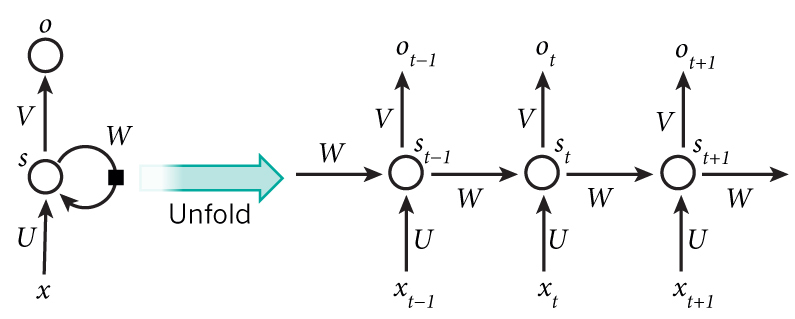
\includegraphics[scale=0.4]{Pictures/rnn.jpg}
		\rule{35em}{0.5pt}
		\caption[Recurrent Neural Network]{Recurrent Neural Network. \\ The left-hand side of the figure shows the unfolded version of a simplistic RNN, the black box on the self edge on the state node shows the addition of a time delay, thereby allowing the unfolding based on the time index of each input/ouput pair in the sequence.}
		\label{fig:rnn}
\end{figure}

The equations that correspond to the unfolded computational graph in fig.\ref{fig:rnn} can be stated as follows:
\begin{align*}
\bm{a}^{(t)} &= \bm b + \bm{Wh}^{(t-1)} + \bm{Ux}^{(t)} \\
\bm{h}^{(t)} &= tanh(\bm{a}^{(t)}) \\
\bm{o}^{(t)} &= \bm c + \bm{Wh}^{(t)}
\end{align*}

While training, the error is calculated via a loss function (usually \textit{cross-entropy loss}) by the following equation,
\begin{equation}
\hat{\bm y}^{(t)} = softmax(\bm{o}^{(t)})
\end{equation}
\subsection*{Training in RNNs}
Traditional backpropagation is evidently not possible for computing the gradients in an unfolded, due to the setup of the network. A modified version of the algorithm is required. It is called \textit{back-propagation over time} (BPTT) algorithm. THe calculation of the gradient starts at the last time step $\tau$ and propagates backward for each time step $t$. The original gradient will be,
\begin{align*}
\frac{\partial L}{\partial L^{(t)}} &= 1 \\
\left(\nabla_{\bm{o}^{(t)}}L\right)_{i} &= \hat{\bm{y}}_{i}^{(t)} - \bm 1 _{i,y^{(t)}} \\
\nabla_{\bm{h}^{(t)}}L &= \left(\frac{\partial \bm{h}^{(t+1)}}{\partial \bm{h}^{(t)}} \right) ^{\top}(\nabla_{\bm{h}^{(t+1)}}L) + \left(\frac{\partial \bm{o}^{(t)}}{\partial \bm{h}^{(t)}} \right) ^{\top} (\nabla_{\bm{o}^{(t)}}L)
\end{align*}
\section{High-Dimension Statistics}
\label{sec:highds}
In this section we address some the observations on the behaviour of multiple instances of networks and draw some statistical understanding on the reasons behind these behaviours. We use this information to analyse how these properties can be advantageous (or not) and how desirable properties can be created in networks.




% Chapter 1

\chapter{Implementation} % Main chapter title

\label{implement} % For referencing the chapter elsewhere, use \ref{Chapter1} 

\lhead{Chapter 4. \emph{Implementation}} % This is for the header on each page - perhaps a shortened title

%----------------------------------------------------------------------------------------

\section{Abstraction of Subroutines}

\section{Code}
Following is the code for seminal models highly illustrative of the architectures presented in earlier chapters.

\subsection*{AlexNet}
\begin{lstlisting}
################################################################################
#Michael Guerzhoy and Davi Frossard, 2016
#AlexNet implementation in TensorFlow, with weights
#Details: 
#http://www.cs.toronto.edu/~guerzhoy/tf_alexnet/
#
#
################################################################################

from numpy import *
import os
from pylab import *
import numpy as np
import matplotlib.pyplot as plt
import matplotlib.cbook as cbook
import time
from scipy.misc import imread
from scipy.misc import imresize
import matplotlib.image as mpimg
from scipy.ndimage import filters
import urllib
from numpy import random


import tensorflow as tf

from caffe_classes import class_names

train_x = zeros((1, 227,227,3)).astype(float32)
train_y = zeros((1, 1000))
xdim = train_x.shape[1:]
ydim = train_y.shape[1]

################################################################################
#Read Image

im1 = (imread("poodle.png")[:,:,:3]).astype(float32)
im1 = im1 - mean(im1)

im2 = (imread("laska.png")[:,:,:3]).astype(float32)
im2 = im2 - mean(im2)

################################################################################

net_data = load("bvlc_alexnet.npy").item()

def conv(input, kernel, biases, k_h, k_w, c_o, s_h, s_w,  padding="VALID", group=1):
    '''From https://github.com/ethereon/caffe-tensorflow
    '''
    c_i = input.get_shape()[-1]
    assert c_i%group==0
    assert c_o%group==0
    convolve = lambda i, k: tf.nn.conv2d(i, k, [1, s_h, s_w, 1], padding=padding)
    
    
    if group==1:
        conv = convolve(input, kernel)
    else:
        input_groups = tf.split(3, group, input)
        kernel_groups = tf.split(3, group, kernel)
        output_groups = [convolve(i, k) for i,k in zip(input_groups, kernel_groups)]
        conv = tf.concat(3, output_groups)
    return  tf.reshape(tf.nn.bias_add(conv, biases), [-1]+conv.get_shape().as_list()[1:])

x = tf.placeholder(tf.float32, (None,) + xdim)


#conv1
k_h = 11; k_w = 11; c_o = 96; s_h = 4; s_w = 4
conv1W = tf.Variable(net_data["conv1"][0])
conv1b = tf.Variable(net_data["conv1"][1])
conv1_in = conv(x, conv1W, conv1b, k_h, k_w, c_o, s_h, s_w, padding="SAME", group=1)
conv1 = tf.nn.relu(conv1_in)

#lrn1
#lrn(2, 2e-05, 0.75, name='norm1')
radius = 2; alpha = 2e-05; beta = 0.75; bias = 1.0
lrn1 = tf.nn.local_response_normalization(conv1,
                                                  depth_radius=radius,
                                                  alpha=alpha,
                                                  beta=beta,
                                                  bias=bias)

#maxpool1
k_h = 3; k_w = 3; s_h = 2; s_w = 2; padding = 'VALID'
maxpool1 = tf.nn.max_pool(lrn1, ksize=[1, k_h, k_w, 1], strides=[1, s_h, s_w, 1], padding=padding)


#conv2
k_h = 5; k_w = 5; c_o = 256; s_h = 1; s_w = 1; group = 2
conv2W = tf.Variable(net_data["conv2"][0])
conv2b = tf.Variable(net_data["conv2"][1])
conv2_in = conv(maxpool1, conv2W, conv2b, k_h, k_w, c_o, s_h, s_w, padding="SAME", group=group)
conv2 = tf.nn.relu(conv2_in)


#lrn2
radius = 2; alpha = 2e-05; beta = 0.75; bias = 1.0
lrn2 = tf.nn.local_response_normalization(conv2,
                                                  depth_radius=radius,
                                                  alpha=alpha,
                                                  beta=beta,
                                                  bias=bias)

#maxpool2                                               
k_h = 3; k_w = 3; s_h = 2; s_w = 2; padding = 'VALID'
maxpool2 = tf.nn.max_pool(lrn2, ksize=[1, k_h, k_w, 1], strides=[1, s_h, s_w, 1], padding=padding)

#conv3
k_h = 3; k_w = 3; c_o = 384; s_h = 1; s_w = 1; group = 1
conv3W = tf.Variable(net_data["conv3"][0])
conv3b = tf.Variable(net_data["conv3"][1])
conv3_in = conv(maxpool2, conv3W, conv3b, k_h, k_w, c_o, s_h, s_w, padding="SAME", group=group)
conv3 = tf.nn.relu(conv3_in)

#conv4
k_h = 3; k_w = 3; c_o = 384; s_h = 1; s_w = 1; group = 2
conv4W = tf.Variable(net_data["conv4"][0])
conv4b = tf.Variable(net_data["conv4"][1])
conv4_in = conv(conv3, conv4W, conv4b, k_h, k_w, c_o, s_h, s_w, padding="SAME", group=group)
conv4 = tf.nn.relu(conv4_in)


#conv5
k_h = 3; k_w = 3; c_o = 256; s_h = 1; s_w = 1; group = 2
conv5W = tf.Variable(net_data["conv5"][0])
conv5b = tf.Variable(net_data["conv5"][1])
conv5_in = conv(conv4, conv5W, conv5b, k_h, k_w, c_o, s_h, s_w, padding="SAME", group=group)
conv5 = tf.nn.relu(conv5_in)

#maxpool5
k_h = 3; k_w = 3; s_h = 2; s_w = 2; padding = 'VALID'
maxpool5 = tf.nn.max_pool(conv5, ksize=[1, k_h, k_w, 1], strides=[1, s_h, s_w, 1], padding=padding)

#fc6
fc6W = tf.Variable(net_data["fc6"][0])
fc6b = tf.Variable(net_data["fc6"][1])
fc6 = tf.nn.relu_layer(tf.reshape(maxpool5, [-1, int(prod(maxpool5.get_shape()[1:]))]), fc6W, fc6b)

#fc7
fc7W = tf.Variable(net_data["fc7"][0])
fc7b = tf.Variable(net_data["fc7"][1])
fc7 = tf.nn.relu_layer(fc6, fc7W, fc7b)

#fc8
fc8W = tf.Variable(net_data["fc8"][0])
fc8b = tf.Variable(net_data["fc8"][1])
fc8 = tf.nn.xw_plus_b(fc7, fc8W, fc8b)


#prob
prob = tf.nn.softmax(fc8)

init = tf.initialize_all_variables()
sess = tf.Session()
sess.run(init)

t = time.time()
output = sess.run(prob, feed_dict = {x:[im1,im2]})
################################################################################

#Output:
for input_im_ind in range(output.shape[0]):
    inds = argsort(output)[input_im_ind,:]
    print "Image", input_im_ind
    for i in range(5):
        print class_names[inds[-1-i]], output[input_im_ind, inds[-1-i]]

print time.time()-t
\end{lstlisting}
\subsection*{Char-rnn for sentence creation}
\begin{lstlisting}
# code from https://github.com/sherjilozair/
from __future__ import print_function
import numpy as np
import tensorflow as tf

import argparse
import time
import os
from six.moves import cPickle

from utils import TextLoader
from model import Model

def main():
    parser = argparse.ArgumentParser()
    parser.add_argument('--data_dir', type=str, default='data/tinyshakespeare',
                       help='data directory containing input.txt')
    parser.add_argument('--save_dir', type=str, default='save',
                       help='directory to store checkpointed models')
    parser.add_argument('--rnn_size', type=int, default=128,
                       help='size of RNN hidden state')
    parser.add_argument('--num_layers', type=int, default=2,
                       help='number of layers in the RNN')
    parser.add_argument('--model', type=str, default='lstm',
                       help='rnn, gru, or lstm')
    parser.add_argument('--batch_size', type=int, default=50,
                       help='minibatch size')
    parser.add_argument('--seq_length', type=int, default=50,
                       help='RNN sequence length')
    parser.add_argument('--num_epochs', type=int, default=50,
                       help='number of epochs')
    parser.add_argument('--save_every', type=int, default=1000,
                       help='save frequency')
    parser.add_argument('--grad_clip', type=float, default=5.,
                       help='clip gradients at this value')
    parser.add_argument('--learning_rate', type=float, default=0.002,
                       help='learning rate')
    parser.add_argument('--decay_rate', type=float, default=0.97,
                       help='decay rate for rmsprop')                       
    parser.add_argument('--init_from', type=str, default=None,
                       help="""continue training from saved model at this path. Path must contain files saved by previous training process: 
                            'config.pkl'        : configuration;
                            'chars_vocab.pkl'   : vocabulary definitions;
                            'checkpoint'        : paths to model file(s) (created by tf).
                                                  Note: this file contains absolute paths, be careful when moving files around;
                            'model.ckpt-*'      : file(s) with model definition (created by tf)
                        """)
    args = parser.parse_args()
    train(args)

def train(args):
    data_loader = TextLoader(args.data_dir, args.batch_size, args.seq_length)
    args.vocab_size = data_loader.vocab_size
    
    # check compatibility if training is continued from previously saved model
    if args.init_from is not None:
        # check if all necessary files exist 
        assert os.path.isdir(args.init_from)," %s must be a a path" % args.init_from
        assert os.path.isfile(os.path.join(args.init_from,"config.pkl")),"config.pkl file does not exist in path %s"%args.init_from
        assert os.path.isfile(os.path.join(args.init_from,"chars_vocab.pkl")),"chars_vocab.pkl.pkl file does not exist in path %s" % args.init_from
        ckpt = tf.train.get_checkpoint_state(args.init_from)
        assert ckpt,"No checkpoint found"
        assert ckpt.model_checkpoint_path,"No model path found in checkpoint"

        # open old config and check if models are compatible
        with open(os.path.join(args.init_from, 'config.pkl')) as f:
            saved_model_args = cPickle.load(f)
        need_be_same=["model","rnn_size","num_layers","seq_length"]
        for checkme in need_be_same:
            assert vars(saved_model_args)[checkme]==vars(args)[checkme],"Command line argument and saved model disagree on '%s' "%checkme
        
        # open saved vocab/dict and check if vocabs/dicts are compatible
        with open(os.path.join(args.init_from, 'chars_vocab.pkl')) as f:
            saved_chars, saved_vocab = cPickle.load(f)
        assert saved_chars==data_loader.chars, "Data and loaded model disagree on character set!"
        assert saved_vocab==data_loader.vocab, "Data and loaded model disagree on dictionary mappings!"
        
    with open(os.path.join(args.save_dir, 'config.pkl'), 'wb') as f:
        cPickle.dump(args, f)
    with open(os.path.join(args.save_dir, 'chars_vocab.pkl'), 'wb') as f:
        cPickle.dump((data_loader.chars, data_loader.vocab), f)
        
    model = Model(args)

    with tf.Session() as sess:
        tf.initialize_all_variables().run()
        saver = tf.train.Saver(tf.all_variables())
        # restore model
        if args.init_from is not None:
            saver.restore(sess, ckpt.model_checkpoint_path)
        for e in range(args.num_epochs):
            sess.run(tf.assign(model.lr, args.learning_rate * (args.decay_rate ** e)))
            data_loader.reset_batch_pointer()
            state = sess.run(model.initial_state)
            for b in range(data_loader.num_batches):
                start = time.time()
                x, y = data_loader.next_batch()
                feed = {model.input_data: x, model.targets: y}
                for i, (c, h) in enumerate(model.initial_state):
                    feed[c] = state[i].c
                    feed[h] = state[i].h
                train_loss, state, _ = sess.run([model.cost, model.final_state, model.train_op], feed)
                end = time.time()
                print("{}/{} (epoch {}), train_loss = {:.3f}, time/batch = {:.3f}" \
                    .format(e * data_loader.num_batches + b,
                            args.num_epochs * data_loader.num_batches,
                            e, train_loss, end - start))
                if (e * data_loader.num_batches + b) % args.save_every == 0\
                    or (e==args.num_epochs-1 and b == data_loader.num_batches-1): # save for the last result
                    checkpoint_path = os.path.join(args.save_dir, 'model.ckpt')
                    saver.save(sess, checkpoint_path, global_step = e * data_loader.num_batches + b)
                    print("model saved to {}".format(checkpoint_path))

if __name__ == '__main__':
    main()
\end{lstlisting}




%% Chapter 1

\chapter{Scope and Limitations} % Main chapter title
\label{scopeandlim} % For referencing the chapter elsewhere, use \ref{Chapter1} 

\lhead{Chapter 5. \emph{Scope and Limitations}} % This is for the header on each page - perhaps a shortened title

%----------------------------------------------------------------------------------------

\section{Residual Networks}

\section{Structured Probabilistic Models}

\section{Irregular Graph Learning}






%\input{Chapters/Chapter6}
%\input{Chapters/Chapter7}

%-------------------------------------------------------------------------------
%	THESIS CONTENT - APPENDICES
%-------------------------------------------------------------------------------

\addtocontents{toc}{\vspace{2em}} % Add a gap in the Contents, for aesthetics


\appendix % Cue to tell LaTeX that the following 'chapters' are Appendices

% Include the appendices of the thesis as separate files from the Appendices
% folder
% Uncomment the lines as you write the Appendices

%% Appendix A

\chapter{Appendix Title Here} % Main appendix title

\label{AppendixA} % For referencing this appendix elsewhere, use \ref{AppendixA}

\lhead{Appendix A. \emph{Appendix Title Here}} % This is for the header on each page - perhaps a shortened title

Write your Appendix content here.
%\input{Appendices/AppendixB}
%\input{Appendices/AppendixC}

\addtocontents{toc}{\vspace{2em}} % Add a gap in the Contents, for aesthetics

\backmatter

%-------------------------------------------------------------------------------
%	BIBLIOGRAPHY
%-------------------------------------------------------------------------------

\label{Bibliography}

\lhead{\emph{Bibliography}} % Change the page header to say "Bibliography"

% \printbibliography

\end{document}
